% !TEX root = ../thesis.tex

\chapter{Background}

The proposed approach in this master thesis requires a comprehensive understanding of relevant literature related to document representations, ranking architectures, keyword extraction techniques, and other related areas. This chapter provides a thorough technical background for each component employed in the proposed approach. The chapter is organized into six sections, with each section focusing on the literature associated with a specific technology. In these sections, the most suitable techniques selected for the master thesis are discussed in detail.

\section{Sentence Encoders}
In many \ac{NLP} techniques, text documents are commonly represented using distributed vectors. These vectors are constructed based on word or phrase-level representations and play a vital role in various tasks such as exploratory analysis, text classification, clustering, and text retrieval. Besides phrases, incorporating additional meta-information from parts-of-speech and named entities can further enhance the performance of these tasks. Over the past decade, significant advancements in phrase representations have greatly influenced \ac{NLP} research. This section provides a comprehensive review of different phrase representations documented in the literature, with a focus on highlighting the specific representations used in this master thesis.

\subsection{Document Representations from Word Embeddings}

Word embeddings are vectorized representations of words or phrases. For instance, let's consider a text corpus $C$ consisting of $N$ documents, and the vocabulary size is denoted as $M$. In this context, each document is represented as $D$, and individual terms are represented as $t$.

\centerline{$C$ = $\{D_1, D_2, D_3,\dots, D_N\}$ }
\centerline{$V$ = $\{t_1, t_2, t_3,\dots, t_M\}$ }

The \ac{BoW} approach, which has been widely used in early studies~\cite{zhao2017fuzzy, qader2019overview}, represents a text document as a feature vector that captures the word frequencies within the document. In this technique, each word corresponds to a dimension in a high-dimensional vector space. This vector space model represents the text in a continuous space~\cite{afzali2019text}. In matrix notation, this representation can be understood as a term-document matrix, as shown in \prettyref{fig:td_matrix}. Each word is represented as a one-hot vector, where only one dimension has a value of one, while the remaining dimensions have values of zero. The frequency of a term $t_i$ in a document $D$ is denoted as $(tf_{t_i})_D$, and the document vectors are represented as $\hat{D}$. However, one of the main drawbacks of this method is the computational complexity when the vocabulary size $M$ of the corpus is large.

\centerline{$\hat{D}$ = $(tf_{t_1}, tf_{t_2}, tf_{t_3},\dots, tf_{t_M})_D$ }

\begin{figure}[h!]
	\centering
	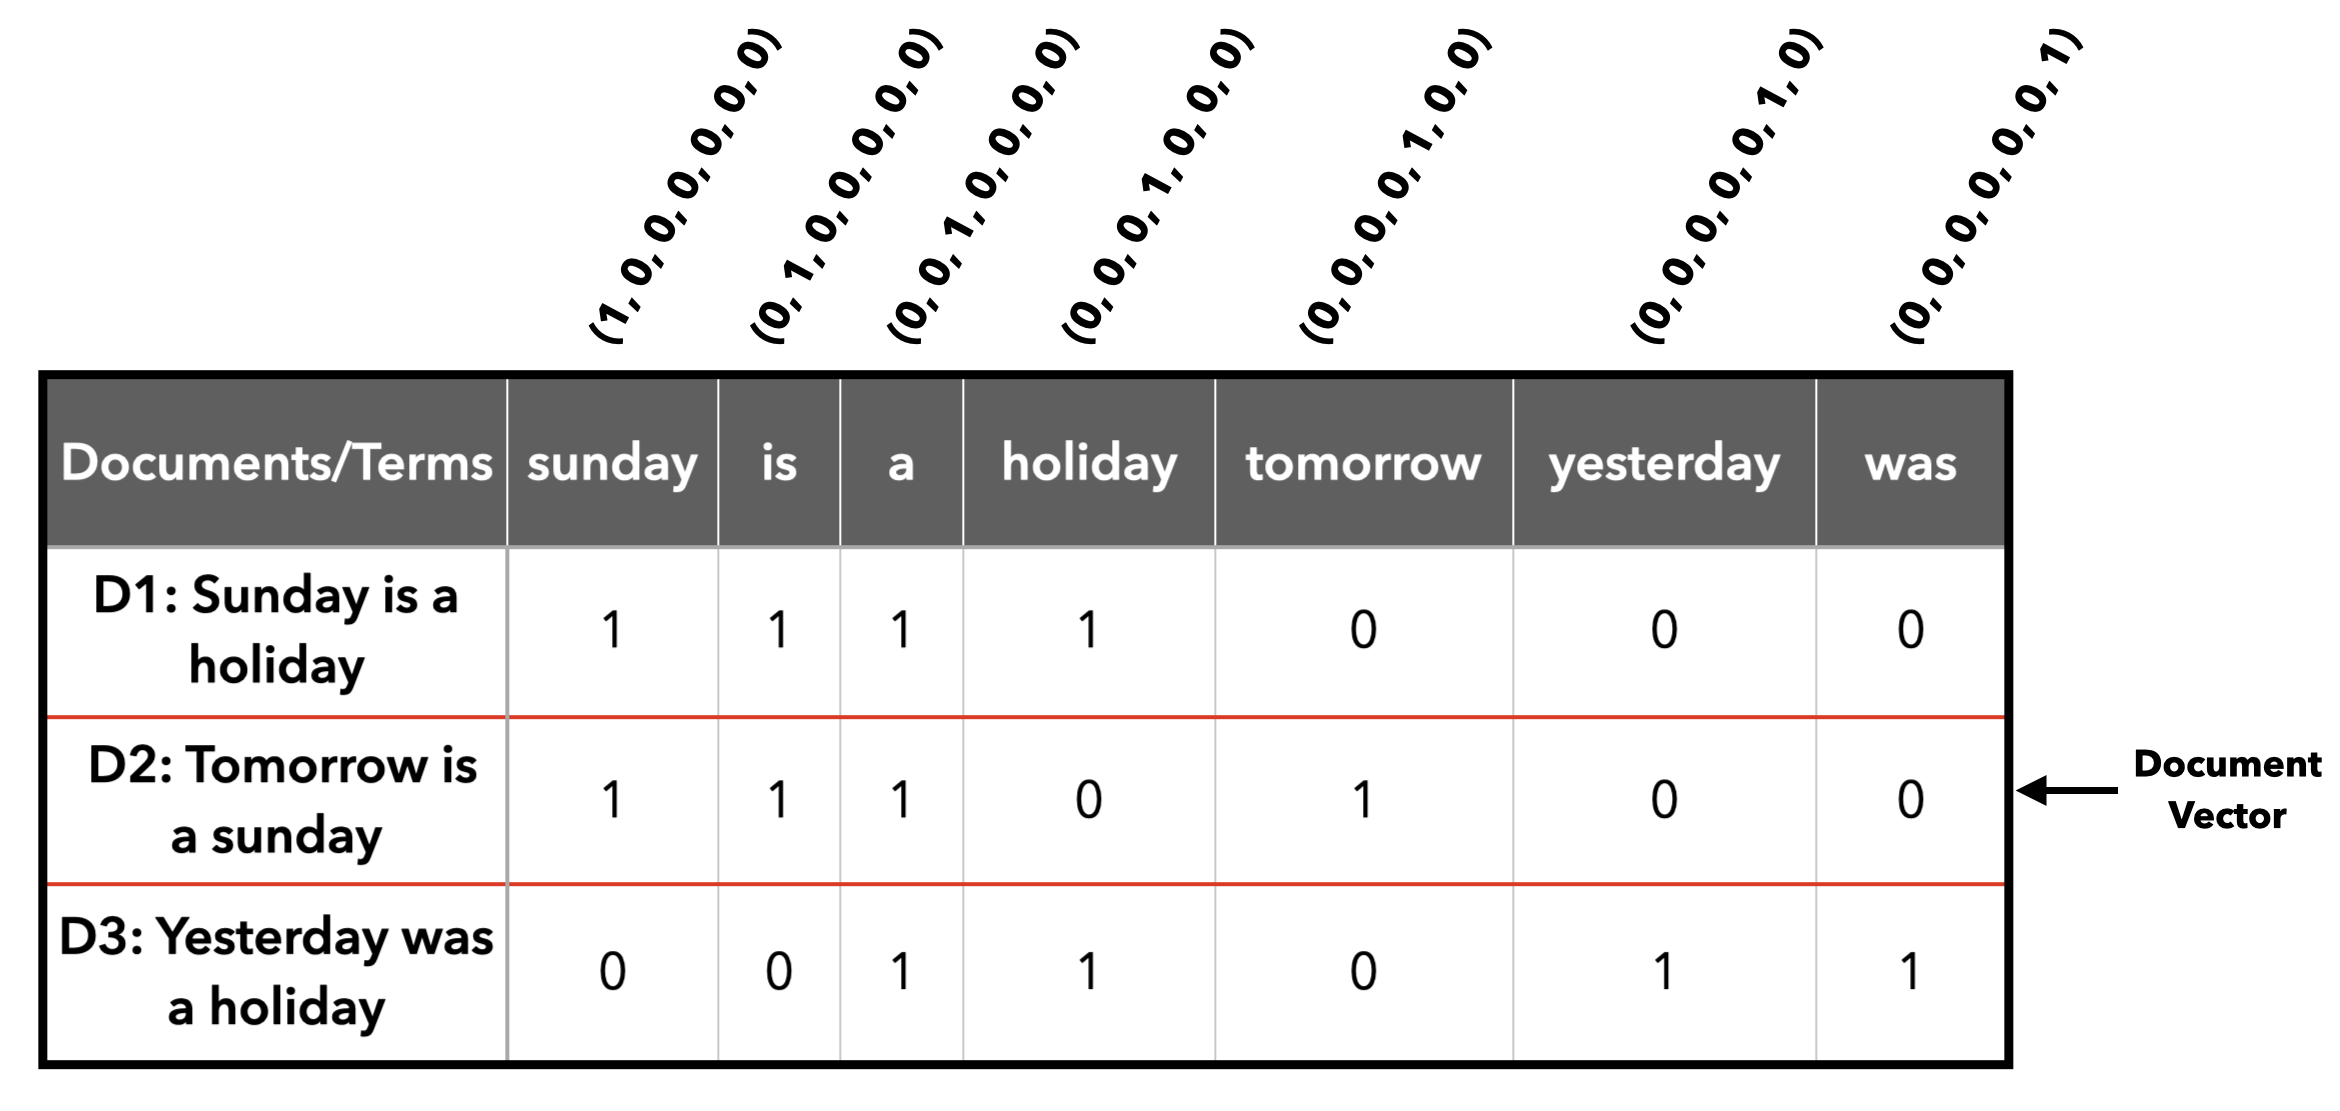
\includegraphics[width=.9\textwidth]{images/thesis_images/term_document_matrix.png}
	\caption[Term-Document matrix example.]{Term-Document matrix representing word and document vectors. \label{fig:td_matrix}}
\end{figure}


To address the limitations of solely relying on word frequency and to take into account the relationship between documents in the corpus, an improved version of the \ac{BoW} approach called \ac{TF-IDF} has been introduced. In this modeling technique, the frequency of a word in all documents across the corpus is taken into consideration, in addition to the term frequencies (or their normalized versions) within individual documents~\cite{lavin2019analyzing}. Terms that appear frequently in many documents are penalized with \ac{TF-IDF}, leading to a more effective weighting score that better reflects their importance in distinguishing documents.

The previous two approaches have limitations as they disregard word order, meaning, and are dependent on the corpus vocabulary. Furthermore, computational challenges can arise when the vocabulary size reaches millions. However, the emergence of \ac{DL} techniques has revolutionized document representations by addressing these limitations. This improvement is achieved through the utilization of semantic word representations that consider word meanings and embed vectors in a continuous vector space, rather than a discrete vector denoting a single dimension~\cite{mikolov2013efficient, pennington2014glove}. These advancements have significantly enhanced the quality of document representations.

Tomas Mikolov et al.~\cite{mikolov2013efficient} proposed an unsupervised training approach involving two model architectures for generating high-quality semantic word vectors. These architectures, known as the \ac{CBOW} and continuous skip-gram models, treat a text document as a continuous sequence of words and uses a window of words. These models operate by considering either the context words or the current word at a given time. A window is defined, spanning the length of the context words. The \ac{CBOW} architecture predicts the probability of the current word given the surrounding context words, while the skip-gram architecture predicts the probability of context words given the current word~\cite{mikolov2013efficient}. Words sharing the same context in the corpus are represented in close proximity to each other within the continuous vector space. Both architectures use a 2-layer feed-forward neural network to generate distributed representations for all words in the corpus. A projection layer is used during tuning instead of a non-linear hidden layer, which is shared across all words.


The above architectures have shown great results representing the semantics of the words. For instance, the vector equation ``king - man + woman = queen'' shows the advancement of word representations in the vector space. However, these architectures primarily focus on local context, which refers to the relationships between words that occur together within a given context or co-occurrences. The consideration of global context is lacking in both the \ac{CBOW} and skip-gram architectures. To address this limitation, Pennington et al.~\cite{pennington2014glove} proposed an approach called \ac{GloVe}. \ac{GloVe} is an unsupervised algorithm that generates distributed word representations by leveraging both local and global word-word co-occurrences. It employs a global log-bilinear regression model that combines techniques of global matrix factorization and local context window. \ac{GloVe} embeddings have exhibited superior performance compared to \ac{CBOW} and other models in tasks such as named entity recognition and word similarity~\cite{pennington2014glove}.

Polysemy refers to the phenomenon where a word or sign has multiple meanings. For example, the word "bank" can represent various concepts such as a river bank or a financial institution. Polysemy creates a significant challenge in both the Word2Vec and \ac{GloVe} approaches as they ignore the possibility of words having different semantics. To tackle this issue, the concept of contextual word embeddings was introduced by \ac{ELMo}~\cite{peters2018deep}. \ac{ELMo} word representations are generated based on the complete sentence rather than a fixed window context. Additionally, word embeddings are derived from the internal states of a bidirectional Language Model (biLM)~\cite{peters2018deep}. \ac{ELMo} also incorporates character convolutions, allowing the model to handle word representations for out-of-vocabulary words. However, Jacob Devlin et al.~\cite{devlin2018bert} argued that the \ac{ELMo} token representations generated by combing left-to-right and right-to-left biLM representations lack deep bidirectionality.


To generate deeply bidirectional word representations, an approach named \ac{BERT} ~\cite{devlin2018bert} is proposed. \ac{BERT} utilizes the transformer architecture which incorporates multi-head attention to efficiently compute embeddings in a vector space. The transformer architecture uses a self-attention mechanism with an encoder-decoder structure to generate input and output representations~\cite{vaswani2017attention}. In its pre-training phase, \ac{BERT} utilizes two techniques: \ac{MLM} and \ac{NSP}. \ac{MLM} randomly masks tokens from the input sequence and predicts the probability of the missing tokens based on their context. This random masking allows \ac{BERT} to produce truly deep bidirectional representations~\cite{devlin2018bert}. Additionally, the \ac{NSP} technique creates sentence pairs and jointly pre-trains the representations of these text pairs by predicting the next sentence given a particular sentence.


\subsection{Sentence Embeddings}

Sentence embeddings serve as numerical representations of text documents, such as sentences or paragraphs. These representations have a significant importance in \ac{IR} particularly in semantic search. A simple approach to generate sentence embeddings involves computing the mean vector representation of the words within a sentence or paragraph (with stopwords removed). However, this approach lacks the semantic coherence among words and inadequately represents the contextual information in the continuous space. In recent years, several approaches for encoding sentences have been proposed, but this section focuses on discussing two widely recognized techniques.

\begin{description}
	\item [\ac{SBERT}]  \hfill \\ The \ac{BERT} encoder is responsible for generating input representations for a sequence of tokens, which can consist of either a single sentence or two combined sentences~\cite{devlin2018bert}. \ac{BERT} incorporates special tokens to identify specific features within the input sequence. For example, the ``[SEP]'' token is utilized to separate two adjacent sentences. Rather than working on a single sentence level, \ac{BERT} operates on token-level embeddings as input. Consequently in the task of semantic similarity, all possible combinations of sentences must be supplied to the \ac{BERT} network which results in a significant computational burden~\cite{reimers-2019-sentence-bert}. Reimers and Gurevych~\cite{reimers-2019-sentence-bert} have highlighted the drawback of \ac{BERT} in generating independent sentence embeddings.
	
	A modification to the pre-training stage of \ac{BERT} called \ac{SBERT} has been proposed to directly generate sentence representations for a given input sentence. \ac{SBERT} incorporates siamese and triplet networks to update the network weights, resulting in the generation of semantically similar sentence embeddings~\cite{reimers-2019-sentence-bert}. Notably, the pre-training of the \ac{SBERT} model alone is sufficient and does not require any additional inference networks to generate the desired sentence representations. These \ac{SBERT} sentence embeddings can be readily applied in various \ac{NLP} tasks, including semantic text similarity, text classification, and text clustering. The models based on the architecture of \ac{SBERT} can be accessed using the sentence-transformers Python library\footnote{\url{https://pypi.org/project/sentence-transformers/}}.
	
	\item [Universal Sentence Encoder (USE)]  \hfill \\ The \ac{USE} is a pre-trained deep learning model developed by tensorFlow, designed to encode text data such as sentences, phrases, or paragraphs into distributed semantic vectors~\cite{cer2018universal}. Two variants of \ac{USE} models have been proposed based on their performance. One model utilizes the transformer architecture, while the other uses the \ac{DAN}. Similar to \ac{SBERT}, \ac{USE} also enables transfer learning using sentence embeddings and eliminates the need for additional inference. Transfer learning experiments conducted with both architectures have demonstrated that the transformer model outperforms \ac{DAN} across various transfer learning tasks, but it requires higher computational resources.
	
	TensorFlow introduced two new multi-lingual \ac{USE} models that are capable of embedding text from sixteen different languages into a single semantic space~\cite{yang2019multilingual}. One of these models utilizes the transformer architecture, while the other uses a convolutional neural network architecture. The \ac{USE} framework utilizes a multi-task dual encoder training approach and enables the deep learning model to train on multiple languages simultaneously~\cite{yang2019multilingual}. In this master thesis, the \ac{USE} model with the transformer architecture from \emph{Tensorflow Hub}\footnote{\url{https://tfhub.dev/google/universal-sentence-encoder-multilingual-large/3}} is utilized. According to tensorflow hub, this particular \ac{USE} model is optimized for processing multi-word text elements, such as sentences, phrases, or short paragraphs, and it does not require explicit language specification. The proposed approach uses the \ac{USE} model in various ways, including document representation, keyword extraction, and semantic document retrieval. The detailed usage of the \ac{USE} model are further elaborated in the subsequent chapters.

	
\end{description}

\section{Neural Ranking Encoders}

Neural ranking encoders refer to deep learning models that rank documents based on their relevance to a given search query. Among these models, BERT-based neural ranking models have gained significant popularity and are typically categorized into two distinct types: \emph{Bi-encoder} and \emph{Cross-encoder} models~\cite{choi2021improving, jung2022semi, ishihara2022nikkei}. The differentiation between these models lies in the encoding process of both the search query and the documents. \prettyref{fig:neural_reranker} illustrates the architectural differences between these two models.

\begin{figure}[h]
	\centering
	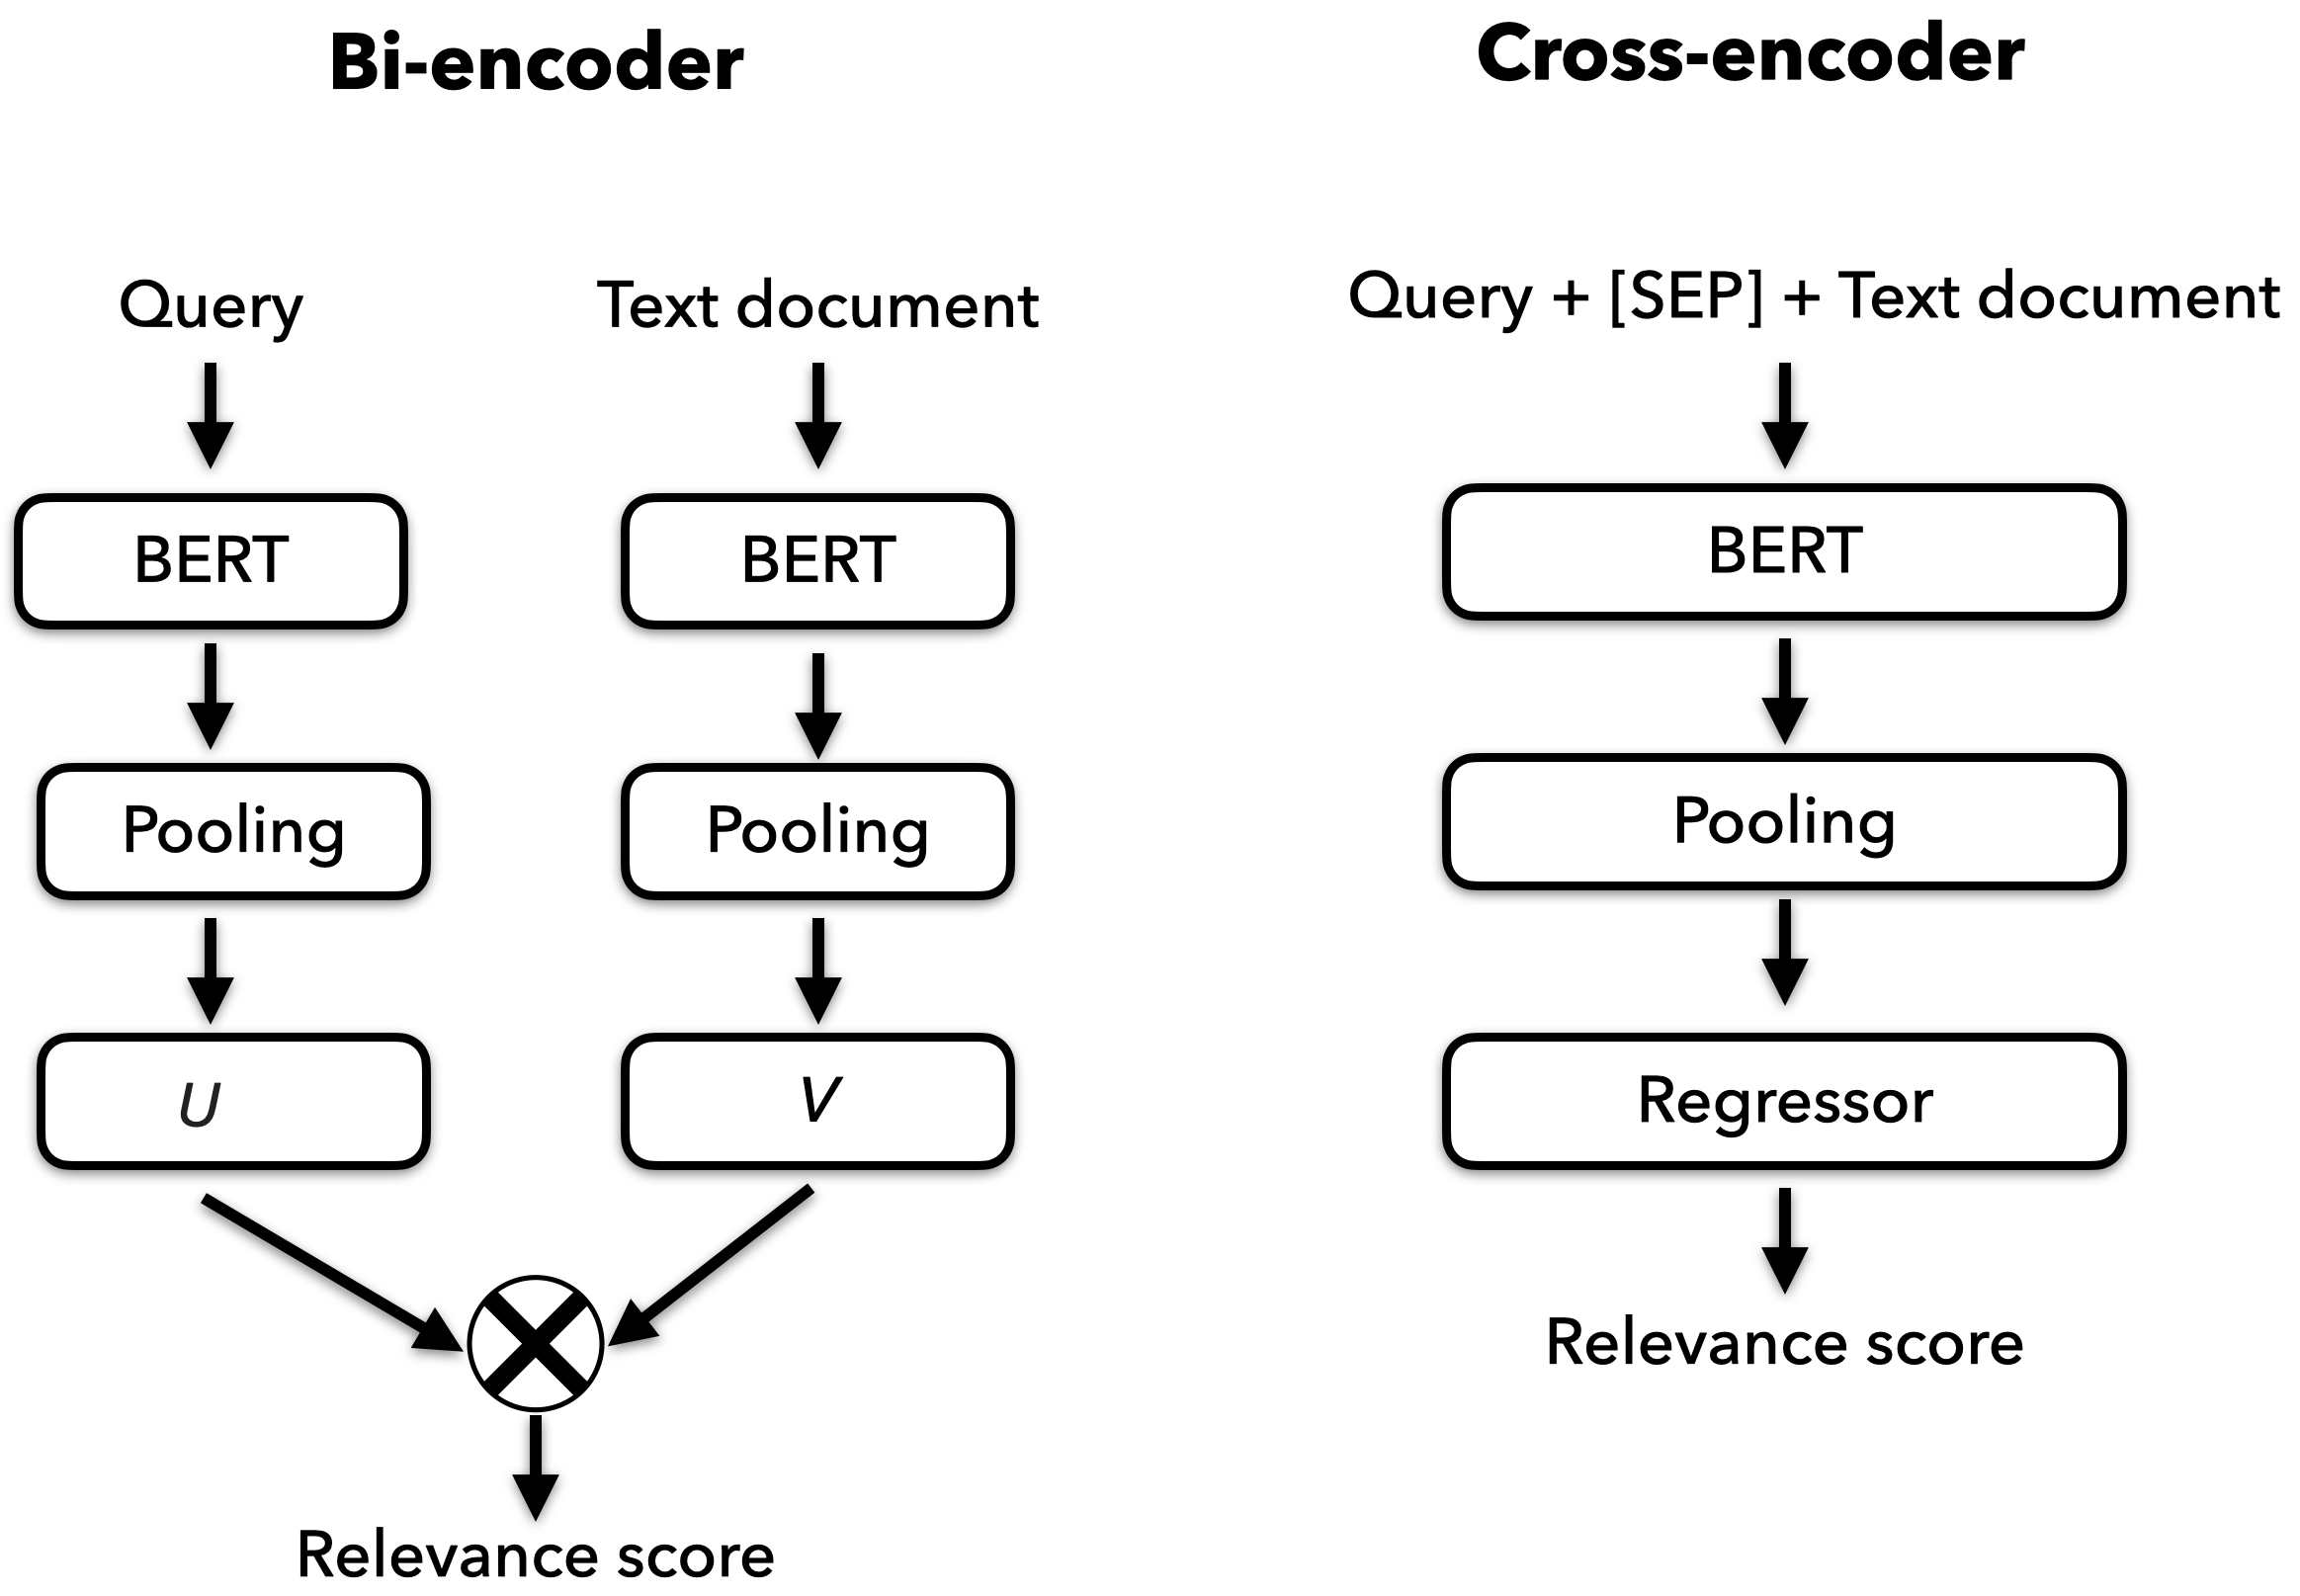
\includegraphics[width=.8\textwidth]{images/thesis_images/neural_ranking_models.png}
	\caption[Bi-encoder and cross-encoder model architectures.]{Bi-encoder and cross-encoder model architectures~\cite{ ishihara2022nikkei}. \label{fig:neural_reranker}}
\end{figure}

\begin{description}
	\item[Bi-encoder]  \hfill \\ Bi-encoder models are neural network architectures that encode the query and documents independently without considering their contextual relationship. In BERT-based bi-encoder networks, separate self-attentions are performed for the query and documents which results in separate dense representation vectors for the query and documents~\cite{choi2021improving}. To measure similarity, an external metric like Euclidean distance or cosine similarity must be used.
	 
	\item[Cross-encoder]  \hfill \\ On the other hand, cross-encoder models are neural network architectures that considers the contextual relationship between the query and documents during the encoding process. In BERT-based cross-encoder networks, a full self-attention mechanism is applied to the query and document pair with a separation token (``[SEP]'') between them~\cite{choi2021improving}. Pre-trained cross-encoder models directly assign a relevance score to the query within the range of [-1, 1].
	
\end{description}

Both the above-mentioned ranking models can be used for \ac{IR}, question-answering, and other related tasks. Cross-encoders generally show superior performance compared to bi-encoders, but requires more computational resources for training or fine-tuning~\cite{choi2021improving, jung2022semi}. This master thesis exclusively uses pre-trained BERT-based ranking encoders. Neural ranking models are employed specifically for comparing the proposed approach with existing literature. Further details on the usage of these encoders are provided in subsequent chapters.

\section{Automatic Keyword Extraction}

Beliga~\cite{beliga2014keyword} has described keyword extraction as the automatic identification of terms that best represent the most relevant information in the document. Keyword extraction techniques are mainly classified into unsupervised or supervised approaches~\cite{bennani2018simple}. Supervised keyword extraction approaches require many labeled datasets containing both documents and keywords from each document. Manual annotation of keywords from each document is a very expensive and tedious task~\cite{beliga2014keyword}, depending on the length of the documents. On the other hand, unsupervised approaches do not require any labeled information but often have poor accuracy~\cite{bennani2018simple}.


\begin{figure}[h]
	\centering
	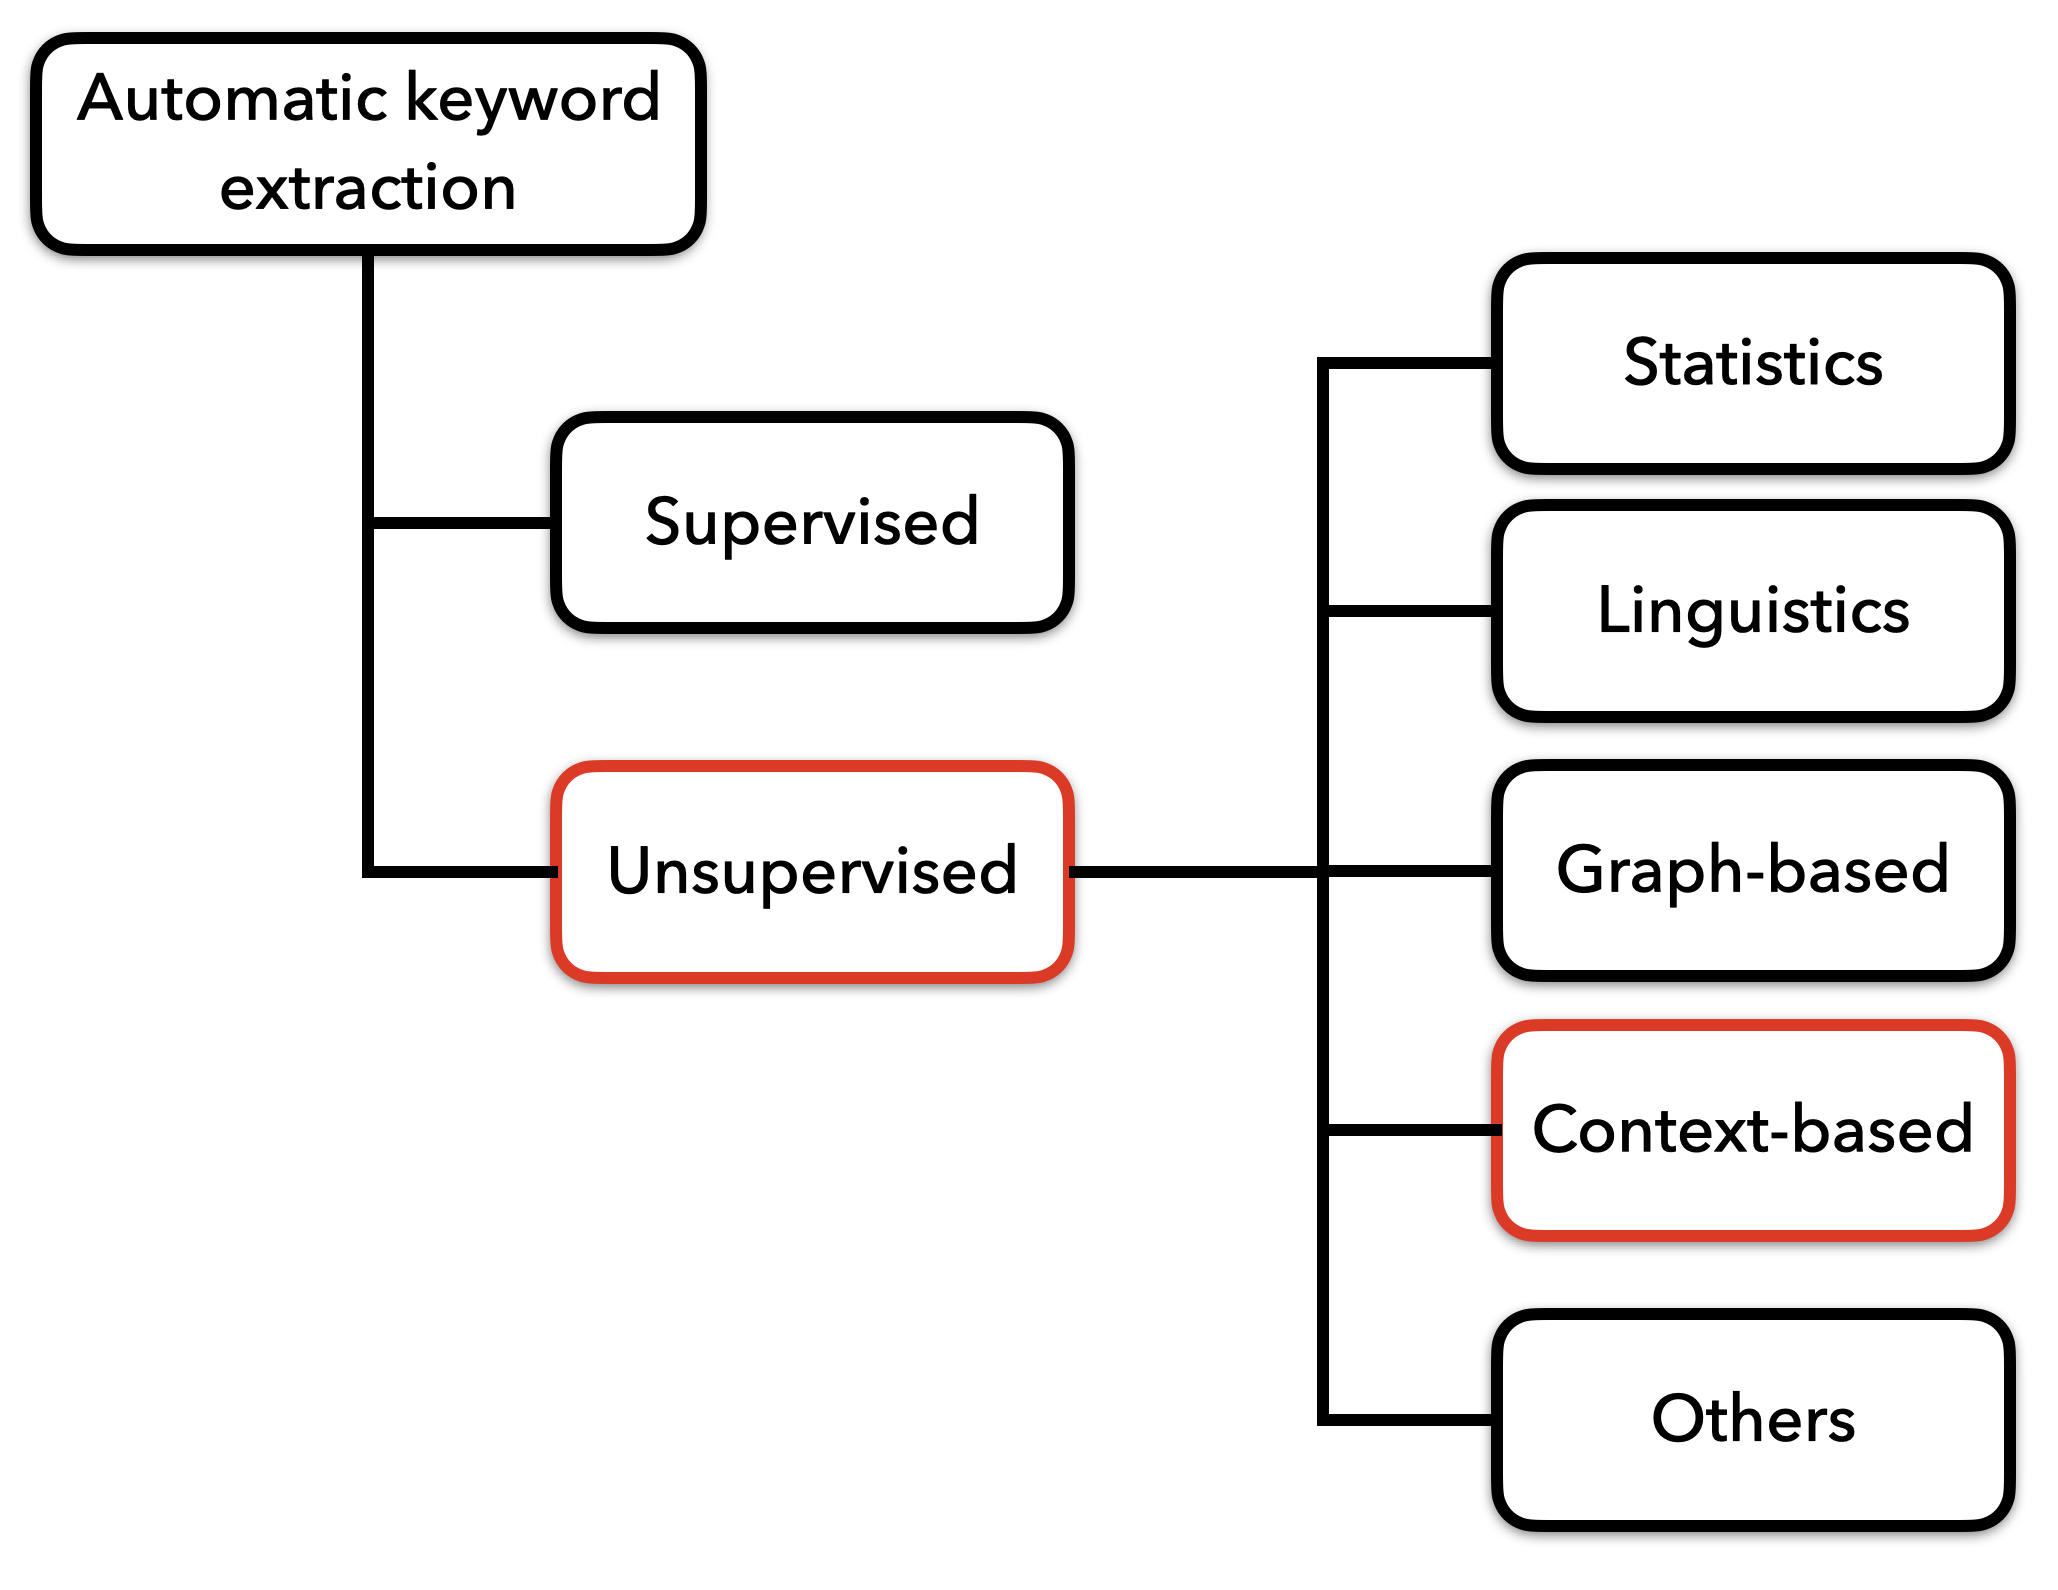
\includegraphics[width=.6\textwidth]{images/thesis_images/keyword_extraction_techniques.png}
	\caption[Keyword extraction techniques.]{Categorization of automatic keyword extraction techniques. \label{fig:keyword_extraction_techniques}}
\end{figure}

Despite the poor accuracy, an unsupervised approach is chosen for extracting keywords in this master thesis as it is difficult and expensive to build a keyword dataset from very long text documents. Some of the popular unsupervised approaches are highlighted in \prettyref{fig:keyword_extraction_techniques}. Statistics-based approaches make use of information such as word frequencies, \ac{TF-IDF}, word co-occurrences, etc.~\cite{beliga2014keyword}. This statistical information is extracted either from an individual document or at the corpus level. Linguistic-based techniques use features that represent the language, such as information related to lexicon, syntax, semantics, etc., to extract keywords~\cite{beliga2014keyword}. On the other hand, graph-based keyword extraction approaches model a document as a graph, where terms are vertices of the graph and the relations between the terms are edges. 

Statistical and linguistic-based features between the terms can be used to represent the edges of the graph. Graph-based approaches perform better than earlier approaches by effectively exploring term relationships~\cite{beliga2014keyword}. In this master thesis, an approach to select keywords based on contextual embeddings is chosen. This approach is inspired by recent research related to using contextualized sentence embeddings for keyphrase extraction, namely \emph{EmbedRank}~\cite{bennani2018simple}. Bennani-Smires et al.~\cite{bennani2018simple} have shown that the EmbedRank approach has performed better than state-of-the-art graph-based keyword extraction approaches. To generate phrase embeddings of the noun chunks and the original news article, a multi-lingual pre-trained \ac{USE} from tensorFlow is employed. 


\section{Dimensionality Reduction}

Sentence or word embeddings are very high-dimensional distributed vectors, especially \ac{USE} embeddings have a dimension size of 512. Data processing tasks such as visualization, data analysis, feature extraction, clustering, etc., on data with high dimensions can be computationally expensive. Therefore, the dimensions of the data are reduced for all the data points in the dataset without losing crucial patterns or information. This technique is generally referred to as dimensionality reduction. Many dimensionality reduction techniques have been proposed in recent years, and they can be categorized into two types. Algorithms that preserve the pairwise distance structure among all the data points in the dataset~\cite{mcinnes2018umap}. One example in this category is \ac{PCA}. \ac{PCA} assumes that the data is linear and does not perform well in the case of data with non-linear relationships. The other type of algorithms considers the non-linear relationships in the data and preserves local or global structures in the data. One example of these non-linear algorithms is \ac{UMAP}.


\begin{figure}[h]
	\centering
	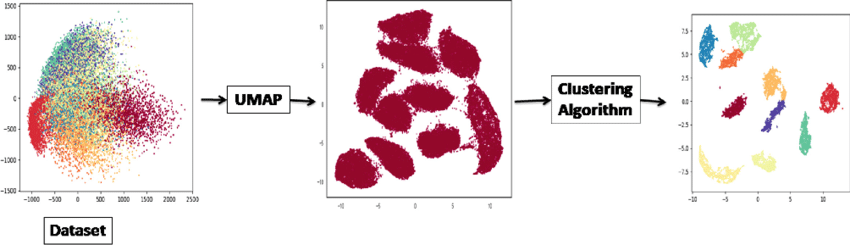
\includegraphics[width=.9\textwidth]{images/papers/umap.png}
	\caption[UMAP pipeline for clustering.]{Improved clustering pipeline after reducing the data dimensions~\cite{allaoui2020considerably}.  \label{fig:umap}}
\end{figure}

Allaoui et al.~\cite{allaoui2020considerably} have observed an increase in the performance of clustering methods after dimensionality reduction on the data using \ac{UMAP}, as shown in \prettyref{fig:umap}. They tested a few popular clustering techniques such as k-means, gaussian mixture models, agglomerative hierarchical clustering, and \ac{HDBSCAN}, and observed an increase in accuracy after \ac{UMAP} dimensionality reduction. Moreover, the time taken for clustering was drastically reduced. \ac{UMAP} works based on \emph{Riemannian geometry and algebraic topology}, preserving the global structure in the data~\cite{mcinnes2018umap}. One of the main reasons for the acceptance of \ac{UMAP} in \ac{ML} is its computational efficiency, though it is slower than \ac{PCA}~\cite{umaplearnPerformanceComparison}. However, given the quality of reduced representations and its ability to handle the non-linear relationships in the data, \ac{UMAP} is clearly a viable dimensionality reduction technique in \ac{ML}. In this master thesis, \ac{UMAP} is used to reduce the dimensionality of the data.



\section{Document Clustering}

\ac{DC} is the task of separating documents into meaningful groups where the documents with similar characteristics belong to a similar group. In addition to \ac{DC}, the task of topic modeling is also referred to in order to achieve the same outcome. \ac{DC} plays a crucial role in the field of big data and data mining. Generally, clustering is performed on numerical data points in the continuous space. However, text documents are in alphanumeric format (including some special characters). One of the earliest approaches to represent text documents is the \ac{BoW} method and \ac{TF-IDF} weighting, which is described in Section 3.1.1. Two main disadvantages of these methods are the lack of semantic representation and high-dimensional representation. Since the dimensions depend on the number of words in the corpus, this can lead to computational overhead. Semantic (contextual) text representations, with the help of word or sentence embeddings, encode the text in fixed-length vectors. There are several clustering techniques tested on text document clustering, such as partitioning, hierarchical, and density-based~\cite{afzali2019text}. Below are a few clustering algorithms discussed at an abstract level, and their advantages and disadvantages are highlighted.


\begin{description}
	
	\item [Partitioning clustering]  \hfill \\ 
	This type of clustering deals with creating a fixed number of clusters of similar data based on a particular criterion. K-means clustering is one of the popular and simple clustering techniques based on distance measurement in \ac{ML}. The K-means algorithm partitions the data of $n$ samples into $k$ clusters using a centroid-based iterative approach~\cite{afzali2019text}. Being a parametric clustering approach, the number of clusters $k$ needs to be well designed according to the data. One major drawback is the cluster shape, as the algorithm expects a spherical or circular shape output due to the centroid approach. K-means also does not assume any inherent noise in the data and assigns all data points to a cluster.
	
	
	\item [Hierarchical clustering]  \hfill \\ These clustering algorithms create a hierarchical structure from the data samples. There are two types of hierarchical clustering methods, namely the top-bottom/divisive approach and the bottom-top/agglomerative approach~\cite{afzali2019text}. In the top-bottom approach, all data samples are considered to be a single cluster, and this cluster is further decomposed into smaller clusters until a certain criterion is achieved. Conversely, in the bottom-top approach, each data sample is considered as a single cluster, and the clusters are merged to form larger clusters until a certain criterion is met~\cite{zhao2002comparison}.
	
	
	Agglomerative hierarchical clustering is one of the popular hierarchical algorithms in \ac{ML}, and unlike k-means, there is no need to specify the number of clusters before clustering. However, extensive experiments comparing both clustering algorithms show that partitioning clustering always performs better than agglomerative clustering~\cite{zhao2002comparison}. The authors also suggest to use partitional clustering for large document collections.

	
	\item [Density based clustering]  \hfill \\ Similar to hierarchical clustering, density-based clustering methods are non-parametric and separate data samples into clusters based on high-density areas until a certain criterion is met. Density can be interpreted as the number of points located within a certain region. \ac{DBSCAN} is one of the popular density-based clustering algorithms. \ac{DBSCAN} characterizes every data point as either a core point, a border point, or a noise point~\cite{campello2020density}. Two crucial parameters in the \ac{DBSCAN} algorithm are $\epsilon$ (epsilon) and $minPts$ (minimum number of points). A data point is defined as a core point when it contains neighboring datapoints higher than $minPts$ within a circle of radius $eps$.
	
	
	\begin{figure}[h]
		\centering
		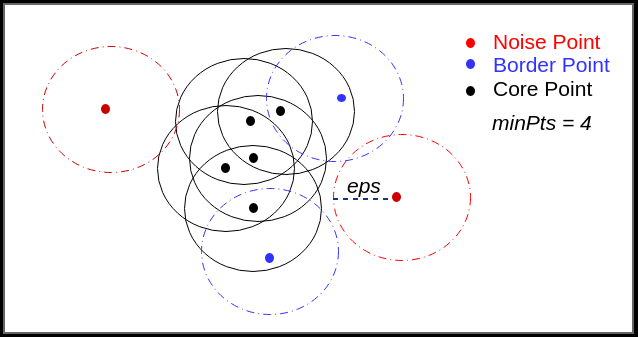
\includegraphics[width=.6\textwidth]{images/papers/dbscan.png}
		\caption[DBSCAN classification of data points.]{DBSCAN classification of data points~\cite{knoldusDBSCANClustering}. \label{fig:dbscan}}
	\end{figure}
	
	A density-based cluster is expressed as a maximally connected component of the data points that lie within a distance less than $eps$ from a core point (as described above)~\cite{campello2020density}. Border points are data points inside a cluster that do not follow the core point property. Data points that are not part of a cluster and do not follow the core point criteria are noise points. Different data points are presented visually in \prettyref{fig:dbscan}. There are more parameters in this algorithm that define the final clustering output, but the number of clusters is not a parameter. This helps the algorithm assign the number of clusters according to the given data.

	
	Density-based clustering clearly has many advantages compared to other clustering algorithms, such as efficient noise handling, non-parametric nature, and flexible clusters (with no specific shape and size). However, \ac{DBSCAN} has limitations, such as difficulty in parameter selection and handling varying density clusters~\cite{mcinnes2017accelerated}. To overcome these limitations, an algorithm called \ac{HDBSCAN} was proposed. This clustering algorithm extends \ac{DBSCAN} by removing the concept of border points and exploring different values of $eps$. 
	
		\begin{figure}[h]
		\centering
		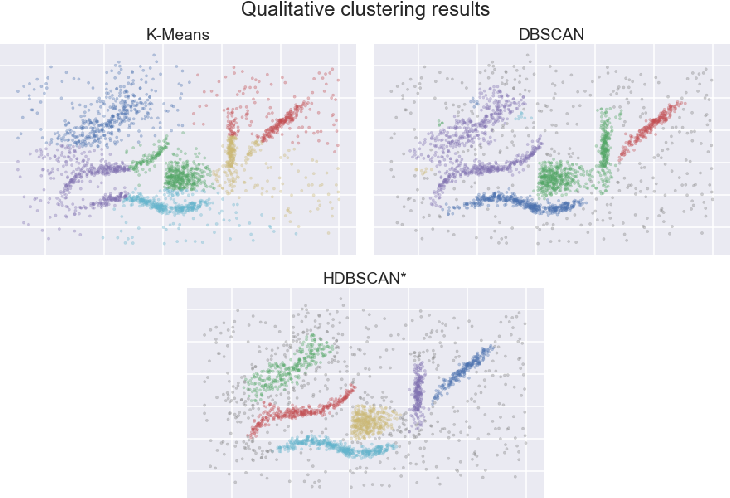
\includegraphics[width=.8\textwidth]{images/papers/hdbscan.png}
		\caption[K-means vs DBSCAN vs HDBSCAN.]{Comparison of clustering results from three algorithms namely k-means, DBSCAN, HDBSCAN~\cite{mcinnes2017accelerated}.  \label{fig:hdbscan}}
	\end{figure}
	
	
	
	A hierarchy of different \ac{DBSCAN} clusterings is generated using different values of $eps$~\cite{mcinnes2017accelerated}. The hierarchy is condensed and used to determine the clustering output, which provides stability for $eps$. To achieve this, a new parameter named \emph{minimum cluster size} is introduced. In this way, \ac{HDBSCAN} overcomes the limitation of handling varying densities, and there is no need to explicitly select the parameter $eps$. In \prettyref{fig:hdbscan}, the results from three clustering algorithms are presented, and it can be observed that \ac{HDBSCAN} handles both low-density noise points and high-density clusters very well. However, \ac{HDBSCAN} is computationally slower compared to \ac{DBSCAN}.

	
	

	
\end{description} 


Clustering algorithms can be further characterized into two types, namely hard clustering and soft clustering, depending on the clustering output~\cite{de2012document}. When the clustering algorithm strictly assigns each data point to a single cluster, it is referred to as \emph{hard clustering}. In \ac{DC}, an example of hard clustering output is when one document is assigned to one cluster. On the other hand, when the clustering output assigns a data point to several clusters, it is referred to as \emph{soft clustering}. For example, when a document is assigned to several clusters, it is an example of soft clustering.


\section{Topic Modeling}

The process of extracting inherent patterns or structures from a large collection of text documents is referred to as \ac{TM}~\cite{angelov2020top2vec}. \ac{TM} is an unsupervised \ac{ML} approach to express a text document as a mixture of topics. For example, a topic can be a general theme such as sports, politics, business, movies, health, etc. \ac{LDA} is one of the popular \ac{TM} algorithms that generates a soft-clustering output. \ac{LDA} is a generative probabilistic model that represents each document as a finite mixture of topics and each topic as a finite mixture of words~\cite{blei2003latent, angelov2020top2vec}. \ac{LDA} uses the \ac{BoW} representation, where a document is a finite set of words. One major limitation of the \ac{LDA} method is the lack of semantic representation.

\begin{figure}[h]
	\centering
	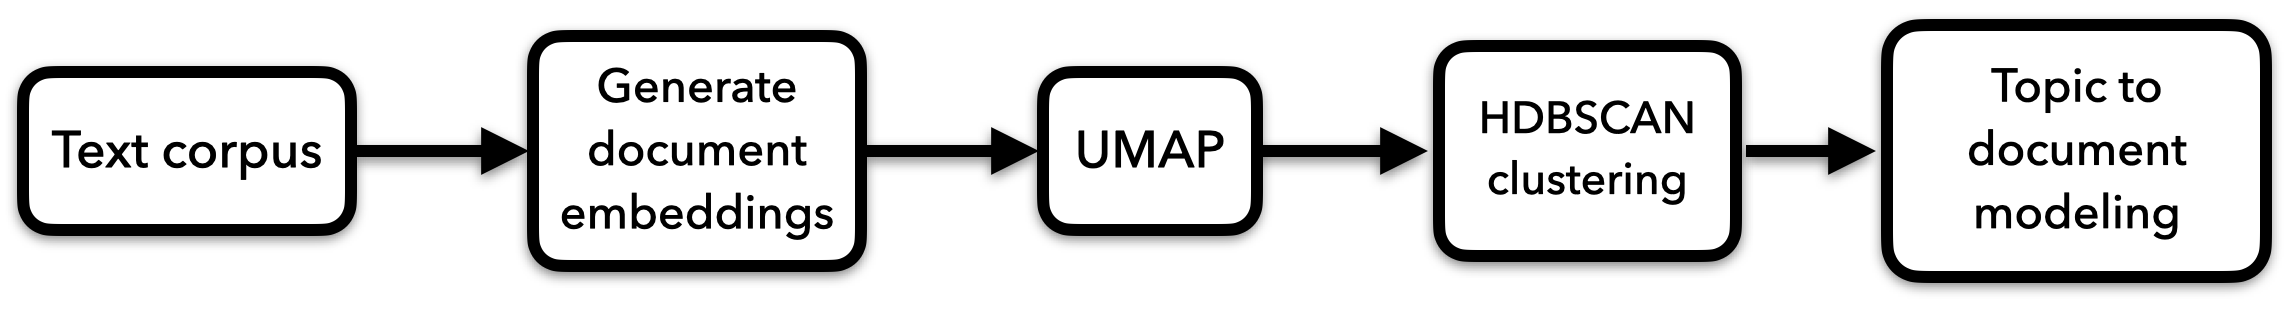
\includegraphics[width=.99\textwidth]{images/thesis_images/top2vec.png}
	\caption[Top2vec topic modeling.]{Top2vec methodology to generate semantic topic-modeling.   \label{fig:top2vec}}
\end{figure}

To overcome this limitation, a new approach called top2vec is proposed. By leveraging the distributed semantic representation of words and sentences, a text document can be represented in the continuous space. This provides an advantage in learning topics in the continuous vector space~\cite{angelov2020top2vec}. top2vec encodes the text documents into the vector space using sentence embeddings. These high-dimensional embeddings are reduced to lower dimensions using the \ac{UMAP} technique and then clustered using the \ac{HDBSCAN} algorithm. The pipeline used in top2vec is presented in \prettyref{fig:top2vec}. During clustering, the high-density areas in the semantic space are grouped together, resulting in topics being expressed as cluster centroids. The results demonstrate that top2vec identifies topics that are more informative and representative compared to the traditional topic modeling algorithm, \ac{LDA}~\cite{angelov2020top2vec}. More details about the technologies and definitions can be found in Appendix \ref{appendix:A}.








